\documentclass[paper=a4, fontsize=11pt]{scrartcl} % A4 paper and 11pt font size

\usepackage[T1]{fontenc} % Use 8-bit encoding that has 256 glyphs
\usepackage[english]{babel} % English language/hyphenation
\usepackage{amsmath,amsfonts,amsthm} % Math packages
\usepackage{graphicx}
\usepackage{sectsty} % Allows customizing section commands
\usepackage{listings}
\usepackage{hyperref}
\usepackage{float}
\usepackage{placeins}
\usepackage{subcaption}
\usepackage{cleveref}
\usepackage{multimedia}

\allsectionsfont{ \normalfont\scshape} % Make all sections centered, the default font and small caps

\usepackage{fancyhdr} % Custom headers and footers
\pagestyle{fancyplain} % Makes all pages in the document conform to the custom headers and footers
\fancyhead{} % No page header - if you want one, create it in the same way as the footers below
\fancyfoot[L]{} % Empty left footer
\fancyfoot[C]{} % Empty center footer
\fancyfoot[R]{\thepage} % Page numbering for right footer
\renewcommand{\headrulewidth}{0pt} % Remove header underlines
\renewcommand{\footrulewidth}{0pt} % Remove footer underlines
\setlength{\headheight}{13.6pt} % Customize the height of the header


%----------------------------------------------------------------------------------------
%	TITLE SECTION
%----------------------------------------------------------------------------------------

\newcommand{\horrule}[1]{\rule{\linewidth}{#1}} % Create horizontal rule command with 1 argument of height

\title{	
\normalfont \normalsize 
\textsc{Indian Institute of Technology Delhi} \\ [25pt] % Your university, school and/or department name(s)
\horrule{0.5pt} \\[0.4cm] % Thin top horizontal rule
\huge Lucas Kanade Tracker \\ % The assignment title
\horrule{2pt} \\[0.5cm] % Thick bottom horizontal rule
}

\author{Suyash Agrawal \\ 2015CS10262} % Your name

\date{\normalsize\today} % Today's date or a custom date

\begin{document}

\maketitle % Print the title

\section{Introduction}
In this assignment we had to implement Lucas Kanade Tracker and using that implement video stabilization
software. The algorithm we used here is Inverse Compositional Algorithm as given in
\textit{Lucas-Kanade 20 Years On: A Unifying Framework} by Baker et al. Here we use the algorithm to compute
the image warp function and we stabilize the video frames using the warp parameters to keep the object at the
same position.

\section{Implementation}
The basic overview of the algorithm is as follows:
\begin{enumerate}
  \item Take an input image and a template image
  \item Compute the gradient, Jacobian, steepest descent and Hessian of the template image
  \item Iterate until marginal increase in warp parameters becomes less than a fixed bound:
  \begin{enumerate}
    \item Warp input image according to initial guess
    \item Compute error in warped image and template image
    \item Calculate the change in warp parameters using the equation in algorithm
    \item Update the warp by composing the marginal change with the previous guess
  \end{enumerate}
\end{enumerate}

\section{Observations}
  We saw the following observations:
  \begin{itemize}
    \item Initial estimate of warp parameters should be close.
    \item The object of interest to stabilize should not exit the window.
    \item The object of interest should be distinctive enough from the background
    \item The lighting conditions must not change drastically during the video.
    \item The template must be carefully selected so that it is unique and gives a good estimate for warp
  \end{itemize}
  
\section{Results}
  \begin{figure*}
    \centering
    \begin{subfigure}[ht]{0.475\textwidth}
        \centering
        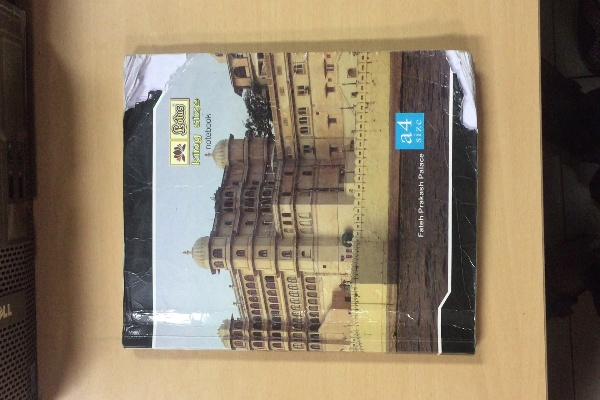
\includegraphics[width=\textwidth]{figures/book_tmpl.jpg}
        \caption{Book Template\label{fig:book_tmpl}}    
    \end{subfigure}
    \vskip\baselineskip
    \begin{subfigure}[ht]{0.475\textwidth}  
        \centering 
        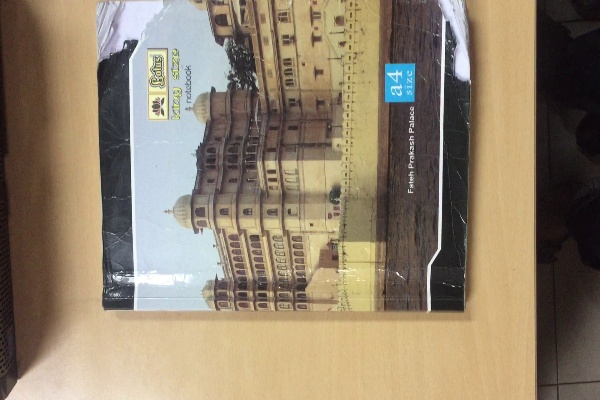
\includegraphics[width=\textwidth]{figures/book_corr.jpg}
        \caption{Shifted Book\label{fig:book_corr}}    
    \end{subfigure}
    \hfill
    \begin{subfigure}[ht]{0.475\textwidth}   
        \centering 
        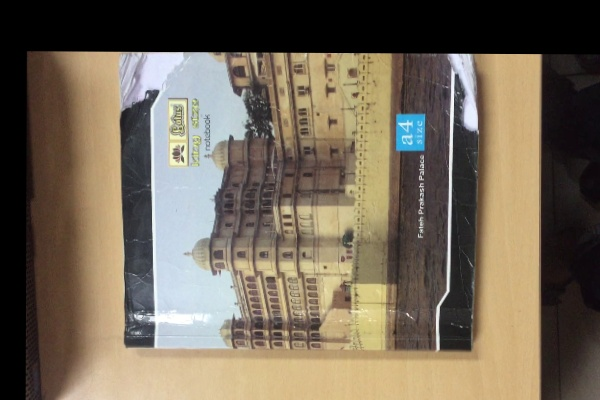
\includegraphics[width=\textwidth]{figures/book_corr_warp.jpg}
        \caption{Warped Shifted Book\label{fig:book_corr_warp}}
    \end{subfigure}

    \vskip\baselineskip
    \begin{subfigure}[ht]{0.475\textwidth}  
        \centering 
        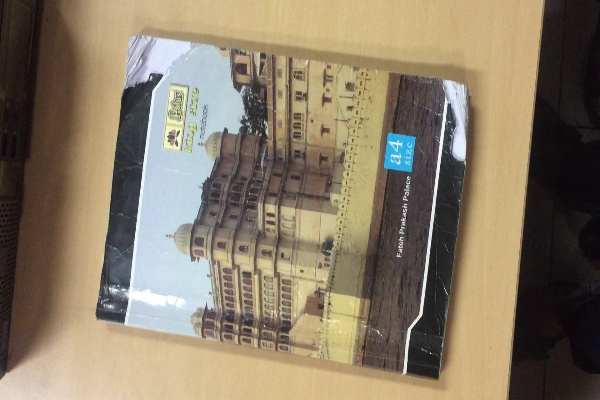
\includegraphics[width=\textwidth]{figures/book_corr_1.jpg}
        \caption{Rotated Book\label{fig:book_corr_1}}    
    \end{subfigure}
    \hfill
    \begin{subfigure}[ht]{0.475\textwidth}   
        \centering 
        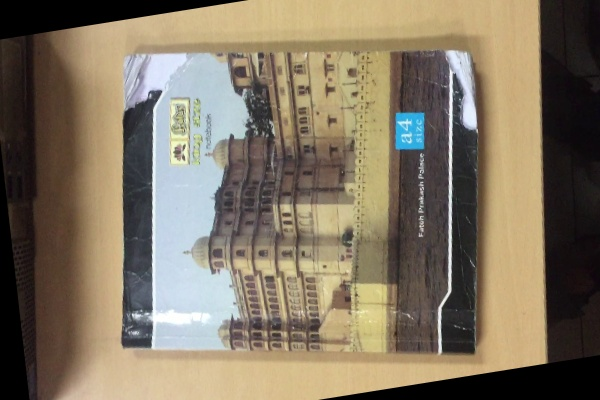
\includegraphics[width=\textwidth]{figures/book_corr_1_warp.jpg}
        \caption{Warped Rotated Book\label{fig:book_corr_1_warp}}
    \end{subfigure}

    \vskip\baselineskip
    \begin{subfigure}[ht]{0.475\textwidth}  
        \centering 
        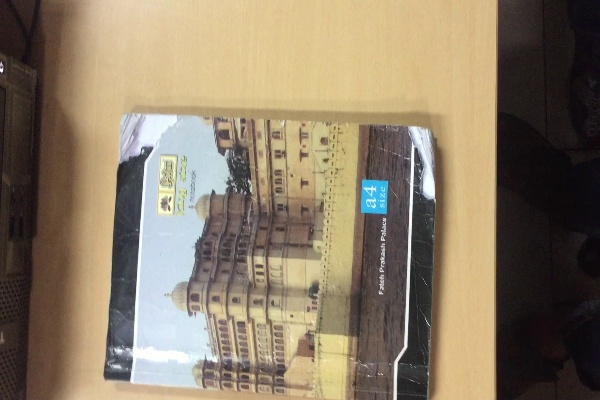
\includegraphics[width=\textwidth]{figures/book_wrong.jpg}
        \caption{Book out of window\label{fig:book_wrong}}    
    \end{subfigure}
    \hfill
    \begin{subfigure}[ht]{0.475\textwidth}   
        \centering 
        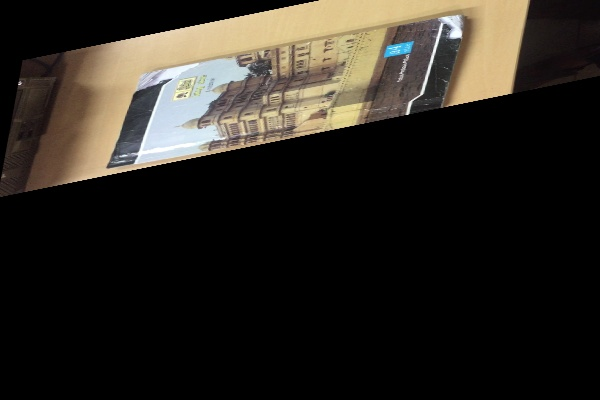
\includegraphics[width=\textwidth]{figures/book_wrong_warp.jpg}
        \caption{Warped image for book out of frame\label{fig:book_wrong_warp}}
    \end{subfigure}

    \caption{Results with Book Video\label{fig:book_video}}
\end{figure*}

The results are computed for two videos: "Shaky Cone"\cite{vid:cone} and "Shaky Book"\cite{vid:book} and the correspoding
result for opencv implementation were also computed.\\
We saw that our implementation was at par with the stabilization by OpenCV and this could be
due to the fact that we explicitly selected an object to stabilize which gave our algorithm
leewage over OpenCV one which didn't had any such object explicitly.

\bibliographystyle{unsrt}
\bibliography{report}

\end{document}